% -----------------------------------------------------------------------------
% -----------------------------------------------------------------------------
%  Universidade Federal do Amazonas
%  Instituto de Computação
%  Ciência da Computação
%
%  Adaptado de pacote abntex2 http://code.google.com/p/abntex2/
%     por Roberto Cidade Fonseca.
% -----------------------------------------------------------------------------
% -----------------------------------------------------------------------------

\documentclass[
	% -- opções da classe memoir --
	12pt,				% tamanho da fonte
	openright,			% capítulos começam em pág ímpar (insere página vazia caso preciso)
	oneside,	
	a4paper,				% tamanho do papel.
	% -- opções da classe abntex2 --
	%chapter=TITLE,		% títulos de capítulos convertidos em letras maiúsculas
	%section=TITLE,		% títulos de seções convertidos em letras maiúsculas
	%subsection=TITLE,		% títulos de subseções convertidos em letras maiúsculas
	%subsubsection=TITLE,	% títulos de subsubseções convertidos em letras maiúsculas
	% -- opções do pacote babel --
	english,				% idioma adicional para hifenização
	brazil				% o último idioma é o principal do documento
]{abntex2/abntex2} % Entre chaves vai o caminho para o arquivo .cls

% ---
% Pacotes básicos
% ---
\usepackage{bookman}				% Usa a fonte Bookman Old Style
\usepackage[T1]{fontenc}			% Selecao de codigos de fonte.
\usepackage[utf8]{inputenc}		% Codificacao do documento (conversão automática dos acentos)
\usepackage{color}				% Controle das cores
\usepackage{graphicx}			% Inclusão de gráficos
\usepackage{microtype} 			% para melhorias de justificação

\usepackage[brazilian,hyper]{backref}	 % Paginas com as citações na bibl
\usepackage[alf]{abntex2cite}	% Citações padrão ABNT
\usepackage{pdfpages} %adicionar documentos pdf. neste caso utilizando no anexo
\usepackage{booktabs} %adicionar tabelas geradas pelo site http://www.tablesgenerator.com

\titulo{Uso de técnicas de \textit{Data Mining} na classificação de sorotipos da dengue}
\autor{Jeferson Barros Alves}
\local{Manaus - AM}
\data{Novembro de 2015}
\orientador[Orientador]{Márcio Palheta Piedade, M.Sc.}
\instituicao{%
  Fundação Centro de Análise, Pesquisa e Inovação Tecnológica
  \par
  Instituto de Ensino Superior Fucapi}
\curso{%
  Coordenação de Graduação em Ciência da Computação}
\tipotrabalho{Monografia}
% O preambulo deve conter o tipo do trabalho, o objetivo, 
% o nome da instituição e a área de concentração 
\preambulo{Monografia apresentada ao Curso de Graduação em Ciência da Computação do Instituto de Ensino Superior FUCAPI - CESF como requisito parcial para a obtenção do Título de Bacharel em Ciência da Computação. Área de concentração: Banco de Dados.}


% Informações do PDF
\makeatletter
\hypersetup{
    	%pagebackref=true,
	pdftitle={\@title}, 
	pdfauthor={\@author},
    	pdfsubject={\imprimirpreambulo},
    pdfcreator={LaTeX with abnTeX2},
	pdfkeywords={abnt}{latex}{abntex}{abntex2}{trabalho acadêmico},
	bookmarksdepth=4
}
\makeatother

% --- 
% Espaçamentos entre linhas e parágrafos 
% --- 

% O tamanho do parágrafo é dado por:
\setlength{\parindent}{1.3cm}

% Controle do espaçamento entre um parágrafo e outro:
%\setlength{\parskip}{0.2cm}  % tente também \onelineskip

%\setbeforesecskip{3em}
%\setbeforesubsecskip{3em}

% ---
% compila o indice
% ---
\makeindex

% ---------------------------------------------------
% INICIO DE DOCUMENTO
% ---------------------------------------------------

\begin{document}

\noindent

% Seleciona o idioma do documento (conforme pacotes do babel)
%\selectlanguage{english}
\selectlanguage{brazil}

% Retira espaço extra obsoleto entre as frases.
\frenchspacing

% ----------------------------------------------------------
% ELEMENTOS PRÉ-TEXTUAIS
% ----------------------------------------------------------
% \pretextual

% ---
% Capa
% ---
\imprimircapa
% ---

% ---
% Folha de rosto
% (o * indica que haverá a ficha bibliográfica)
% ---
\imprimirfolhaderosto*
% ---

% ---
% Inserir folha de aprovação
% ---

% Isto é um exemplo de Folha de aprovação, elemento obrigatório da NBR
% 14724/2011 (seção 4.2.1.3). Você pode utilizar este modelo até a aprovação
% do trabalho. Após isso, substitua todo o conteúdo deste arquivo por uma
% imagem da página assinada pela banca com o comando abaixo:
%
% \includepdf{folhadeaprovacao_final.pdf}
%

%\begin{folhadeaprovacao}
%	\parindent=0pt
%	\setlength{\ABNTEXsignskip}{1.5cm}
%
%	Monografia de Graduação sob o título \textit{Uso de técnicas de Data Mining na classificação de sorotipos da dengue} apresentada por Jeferson Barros Alves e aceita pelo Instituto de Ensino Superior FUCAPI - CESF, sendo aprovada por todos os membros da banca examinadora abaixo especificada:
%
%	\assinatura{\fontsize{12}{15}\selectfont M.Sc. Márcio Palheta Piedade \\ \fontsize{11}{15}\selectfont \imprimirorientadorRotulo}
%	\vspace{1cm}
%	\assinatura{\fontsize{12}{15}\selectfont Titulação e nome do(a) membro da banca examinadora \\ \fontsize{11}{15}\selectfont Co-orientador(a), se houver \\ {\fontsize{10}{12}\selectfont Departamento \par Universidade}}
%	\vspace{1cm}
%	\assinatura{Titulação e nome do membro da banca examinadora \\ {\fontsize{10}{12}\selectfont Departamento \par Universidade}}
%	\vspace{1cm}
%	\assinatura{Titulação e nome do membro da banca examinadora \\ {\fontsize{10}{12}\selectfont Departamento \par Universidade}}
%	\vfill
%    
%	\begin{center}
%		\fontsize{12}{15}\selectfont
%		\vspace*{0.5cm}
%		\imprimirlocal, data de aprovação (por extenso).
%		\vspace*{1cm}
%	\end{center}
%  
%\end{folhadeaprovacao}

% ---
% Dedicatória
% ---
%\begin{dedicatoria}
%   \vspace*{\fill}
%   \noindent
%   \leftskip=5cm

%   Homenagem que o autor presta a uma ou mais pessoas.

%   \vspace{5cm}
%\end{dedicatoria}
% ---

% ---
% Agradecimentos
% ---

%\begin{agradecimentos}

%Agradecimentos dirigidos àqueles que contribuíram de maneira relevante à elaboração do trabalho, sejam eles pessoas ou mesmo organizações.

%\end{agradecimentos}

% ---
% Epígrafe
% ---

%\begin{epigrafe}
%    \vspace*{\fill}
%	\begin{flushright}
%		\textit{Citação}

%		Autor
%	\end{flushright}\vspace{4cm}
%\end{epigrafe}

% ---

% ---
% RESUMOS
% ---

% resumo em português

%\setlength{\absparsep}{18pt} % ajusta o espaçamento dos parágrafos do resumo
%\begin{resumo}

% 	O resumo deve apresentar de forma concisa os pontos relevantes de um texto, fornecendo uma visão rápida e clara do conteúdo e das conclusões do trabalho. O texto, redigido na forma impessoal do verbo, é constituído de uma sequência de frases concisas e objetivas e não de uma simples enumeração de tópicos, não ultrapassando 500 palavras, seguido, logo abaixo, das palavras representativas do conteúdo do trabalho, isto é, palavras-chave e/ou descritores. Por exemplo, deve-se evitar, na redação do resumo, o uso de fórmulas, equações, diagramas e símbolos, optando-se, quando necessário, pela transcrição na forma extensa, além de não incluir citações bibliográficas.

% \textit{Palavras-chave}: Palavra-chave 1, Palavra-chave 2, Palavra-chave 3.

%\end{resumo}

% resumo em inglês

%\begin{resumo}[Abstract]
 %\begin{otherlanguage*}{english}
 %  This is the english abstract.

  % \vspace{\onelineskip}
 
  % \noindent 
  % \textit{Keywords}: Keyword 1, Keyword 2, Keyword 3.
% \end{otherlanguage*}
%\end{resumo}

% ---
% inserir lista de figuras
% ---
\pdfbookmark[0]{\listfigurename}{lof}
\listoffigures*
\cleardoublepage
% ---

% ---
% inserir lista de tabelas
% ---
\pdfbookmark[0]{\listtablename}{lot}
\listoftables*
\cleardoublepage
% ---

% ---
% inserir lista de abreviaturas e siglas
% ---
\begin{siglas}
  \item[KDD] Knowledge Discovery in Databases
  \item[WEKA] Waikato Environment for Knowledge Analysis
  \item[SVM] Support Vector Machine
  \item[SMO] Sequential Minimal Optimization
  \item[SINAN] Sistema de Informação de Agravos de Notificação
\end{siglas}
% ---

% ---
% inserir lista de símbolos
% ---

%\begin{simbolos}
%  \item[$ \lambda $] Lambda
%\end{simbolos}

% ---

% ---
% inserir o sumario
% ---
\pdfbookmark[0]{\contentsname}{toc}
\tableofcontents*
\cleardoublepage
% ---

\textual

\chapter{Introdução}

	Com a grande quantidade de informações geradas e armazenadas por meio do avanço tecnológico das últimas décadas, houve um acúmulo gigantesco de informações. Com isso surgiu uma abordagem de técnicas e ferramentas que buscam transformar dados, denominada Descoberta de Conhecimento em Base de Dados (knowledge Discovery in Databases - KDD), que foi proposto em 1989 com o objetivo de analisar os dados de uma base para que de alguma forma possa ser extraído conhecimento útil \cite{fayyad:1996}.	
	
	A computação tem apoiado o desenvolvimento da medicina em diversas áreas: em sistemas de apoio a coleta de dados clínicos e exames por imagens, na organização das informações obtidas, entre outras. Desta maneira, esse grande volume de dados é uma valiosa fonte de conhecimento que pode ser utilizada para o auxílio ao diagnóstico médico. Assim, é grande a importância do desenvolvimento de técnicas que permitam a descoberta de conhecimento em base de dados médicos para apoiar o médico em sua tarefa diária de tomada de decisões, aumentando a precisão, a confiabilidade e eficiência dos diagnósticos elaborados pelo especialista (COSTA, 2012).
	
	FALAR SOBRE A DENGUE

	\section{Especificação do problema}
	
		\cite{costa:2012} mostrou que o uso de suporte computacional no atendimento médico é comum nos dias de hoje e gera grandes informações digitalizadas dos pacientes. Tais informações armazenadas em base de dados podem representar boas fontes de conhecimento, que pdoerão ser utilizadas no auxílio de diagnóstico médico. Segundo \cite{bezerra:2009}, no passado, o médico detinha conhecimento suficiente para dispensar quase todo o cuidado necessário ao paciente.
		
		Ao longo dos últimos anos a mineração de dados tem sido cada vez mais utilizada na literatura médica. No entanto, a sua aplicação à analise de dados médicos tem sido relativamente limitada, tendo em vista que a aplicação prática pode explorar o conhecimento disponível no contexto clínico e explicar decisões propostas, uma vez que os modelos são utilizados para apoiar decisões \cite{bellazzi:2008}.
		
		É grande a importância do desenvolvimento de técnicas que permitam a descoberta de conhecimento em bases de dados médicos para apoiar o médico em sua tarefa diária de tomada de decisões, aumentando a precisão, a confiabilidade e eficiência dos diagnósticos elaborados pelo especialista \cite{costa:2012}.
		
		A dengue é hoje uma das doenças com maior incidência no Brasil, atingindo a população de todos os estados, independente de classe social. Nesse cenário, torna-se imperioso que um conjunto de ações para a prevenção da doença seja intensificado, permitindo assim a identificação precoce dos casos de dengue, a tomada de decisões e a implementação de medidas de maneira oportuna a fim de principalmente evitar óbitos. Preservar a vida humana é obrigação de todos. "COLOCAR FONTE DO MINISTÉRIO DA SAÚDE"


	\section{Objetivos}

		Construir um classificador que utilize dentre as diversas técnicas de classificação em Data Mining a que mais se adequa ao modelo de dados utilizados na ficha de investigação de dengue do SINAN.
		
		Objetivos Específicos:
		
		\begin{itemize}
			\item Realizar experimentos com classificadores mais utilizados na literatura.

			\item Identificar qual classificador é mais adequado para o trabalho.
			
			\item Utilizar atributos mais relevantes para aplicação da técnica selecionada
			
			\item Tratar o conjunto de dados para aplicação do classificador
			
			\item Construir o modelo classificador
			
			\item Validar e interpretar os resultados obtidos no processo de classificação
		\end{itemize}
		
		Como os objetivos indicam ação, recomenda-se que eles sejam definidos por meio de verbos, tais como analisar, avaliar, caracterizar, discutir, diagnosticar, investigar, implantar, pesquisar, realizar, determinar, etc.
		
	\section{Justificativa}
	
	Na busca constante pela melhoria do atendimento médico hospitalar, as técnicas de mineração de dados estão sendo aplicadas nas bases de dados dos pacientes para descoberta de padrões, seja como ferramenta para auxílio ao diagnóstico ou descobertas que ajudem a alta direção nos hospitais a tomar atitudes com relação aos resultados obtidos (ROBERTINSON, 2012) "DOCUMENTO NÃO ENCONTRADO".
	
	O desenvolvimento de técnicas que permitam a descoberta de conhecimento em bases médicas possui grande importância para apoiar o médico em sua tarefa diária de tomada de decisões, aumentando a precisão, a confiabilidade e a eficiência dos diagnósticos elaborados pelo especialista. Esse apoio computacional pode atuar como uma junta médica virtual, ao trazer para o especialista o conhecimento armazenado em exames e diagnósticos relacionados \cite{costa:2012}.
	
	Com o objetivo de estudo de métodos de suporte ao diagnóstico médico a partir de informações referentes aos sintomas dos pacientes conforme proposto por \cite{alexander:2013}, observamos a necessidade de continuar o trabalho utilizando a técnica de regras de associação em outro conjunto de dados da mesma base.
	
	\section{Trabalhos Relacionados}	
	
	No trabalho de \cite{shakil:2015}, observamos que o foco principal do trabalho foi a classificação de dengue, onde inicialmente aplicou-se a classificação nos datasets iniciais para identificar qual algoritmo obteve melhor resultado. O experimentos releram que os algoritmos Naive Bayes e J48 obtiveram melhores resultados, onde as maiores contribuições do trabalho foram:
	
	\begin{itemize}
		\item A extração da acurácia de classificação para predição do diagnóstico de dengue.
		\item Comparação de diferentes algoritmos de mineração no conjunto de dados de dengue.
		\item Identificar os algoritmos com melhor desempenho para previsão dos diagnósticos.
	\end{itemize}
	
	No trabalho de \cite{thitiprayoonwongse:2012}, foi utilizado a técnica de classificação conhecida como Árvore de Decisão, aplicado a um conjunto de dados temporais contendo dados clínicos e laboratoriais. Utilizaram dois conjuntos de dados com mais de 400 atributos. Nos experimentos os dados foram divididos em: conjunto de teste e treinamento. Onde o objetivo principal deste trabalho foi identificar o dia zero da dengue, pois esta previsão torna-se crítica, tendo em vista que o dia zero tem forte relação com o melhor tratamento do paciente.
	

	No trabalho \cite{santos:2011}, foi desenvolvido um aplicativo para interação dos profissionais da saúde com os dados do SINAN. Onde resultou uma aplicação em java que implementa algoritmos de classificação e regras de associação da base de dados do SINAN utilizando a API WEKA. Como resultado esta ferramente possibilitou o auxílio no diagnóstico de pacientes.

	\section{Metodologia de Desenvolvimento}
		
		Com base na metodologia utilizada no processo de Descoberta de Conhecimento em Base de Dados (Knowledge Dicovery in Databases), a realização desta pesquisa será composta das seguintes etapas:
		
		\begin{itemize}
			\item A primeira etapa deste trabalho baseada na revisão bibliográfica da literatura relacionada a mineração de dados, para determinar outras pesquisas similares a esta, onde são aplicadas as técnicas de mineração de dados em base de dados médicos para descoberta de conhecimento novo e relevante, que de alguma forma possa auxiliar em diagnósticos do médico especialista.
			
			\item Na segunda etapa, ocorrerá a extração, manutenção e pré-processamento dos dados, onde realizaremos a análise de base de dados para extração de informações de atendimentos de pacientes necessários à pesquisa. Em todos os dados ocorrerá um processo de normalização, onde os sintomas relacionados serão dispostos em uma única linha e nos dados ausentes o preenchimento será realizado de forma padrão utilizando o sinal de "?".
			
			\item Na quarta etapa, pode-se executar algoritmos para descoberta do que mais se aproxima do esperado e na extração de informações propriamente dita. O objetivo desta etapa será encontrar padrões na base de dados que foi pré-processada, utilizando a ferramenta de mineração de dados WEKA, um software open-source amplamente utilizado por implementar diversos algoritmos de mineração de dados \cite{hall:2009}.
			
			\item A quinta e última etapa do processo ocorrerá a análise dos resultados obtidos com a a aplicação dos algoritmos de mineração de dados. Encontrar padrões de classificação que sejam relevantes para a pesquisa em questão.
			
		\end{itemize}
		
	\section{Estruturação da Monografia}
	
		Além deste capítulo introdutório, este trabalho está organizado da forma descrita à seguir. No Capítulo 2, descrevemos conceitos básicos relacionados a compreensão deste trabalho, bem como referencial teórico. No Capítulo 3, apresentaremos os experimentos juntamente com os resultados obtidos. Finalmente no Capítulo 4, apresentaremos as conclusões observadas e sugestões de trabalhos futuros da pesquisa.

% ---
% Capítulo 2
% ---
\chapter{Referencial Teórico}

Neste capítulo apresenta-se uma visão geral dos conceitos e procedimentos envolvidos em KDD e consequentemente em Data Mining. Apresentam-se também os trabalhos encontrados na literatura sobre assunto que são relevantes para o desenvolvimento deste trabalho.

	\section{Descoberta de Conhecimento em Base de Dados}
	
	Segundo \cite{fayyad:1996}, a Descoberta de Conhecimento em Base de Dados é um processo não trivial de identificações de novos padrões, válidos e potencialmente úteis.
	
	Em contrapartida, no trabalho de \cite{thome:2002}, define-se KDD como sendo a busca de extração de conhecimento de bases de dados utilizando-se de técnicas e algoritmos que realizam a mineração dos dados para trabalhar e descobrir relações.
	
	O processo de descoberta de conhecimento ocorre quando ocorre um conjunto de padrões que são semelhantes, e que podem levar a construção de um modelo. Este processo é formado por 5 etapas: seleção, pré-processamento, transformação, a mineração de dados e a interpretação dos dados \cite{fayyad:1996}. Além do processo, o conhecimento que se deseja buscar deve estar de acordo com três características: deve ser correto, deve ser compreensível para o usuário e deve ter de alguma forma utilidade para o usuário \cite{freitas:2000}.
	
	A seguir serão detalhadas as etapas do processo de KDD de acordo com o apresentado na figura 1.
	
	A etapa de seleção dos dados inicia com a definição do objetivo e mapeamento  dos grupos ou conjuntos de informações que serão utilizados.
	
	O pré-processamento é responsável pelo tratamento de ruídos e dados incompletos.
	
	A transformação tem como objetivo selecionar as principais características que serão utilizadas para representar os dados, ou seja, os dados devem ser selecionados de  modo que sejam os mais úteis para o modelo proposto.
	
	A etapa de mineração de dados é o momento em que serão escolhidos os  algoritmos que mais se ajustam ao objetivo que se quer extrair da base de dados. Além disso, nesta fase são escolhidos os melhores parâmetros para que, no momento do processamento, os resultados sejam os mais rápidos e precisos possíveis.
	
	Ao final do processo teremos a etapa de interpretação e avaliação dos resultados, onde o conhecimento extraído da base de dados é representado por padrões.
\\
		\begin{figure}[h!]
			\caption{\label{figDataMiningFayyad} Etapas do processo KDD.}
			\begin{center}
			    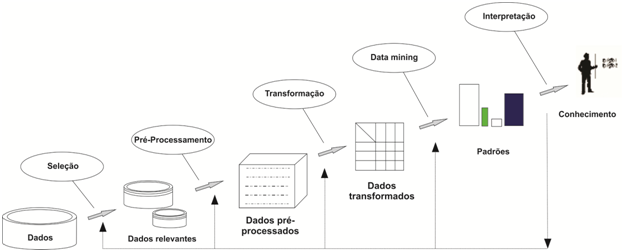
\includegraphics[scale=1]{img/dataMiningFayyad.png}
			    %			    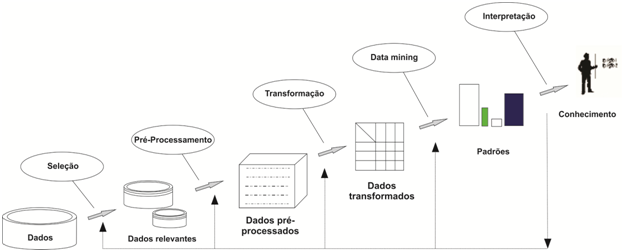
\includegraphics[scale=0.5]{img/dataMiningFayyad}
			\end{center}
			Fonte: \cite{fayyad:1996}.
		\end{figure}
		
		Inicialmente, é necessário definir que tipo de conhecimento se deseja extrair da base de dados, pois a técnica que será utilizada para a mineração de dados depende do objetivo a que se quer chegar \cite{damasceno:2005}.
		
	\section{Data Mining}
	
		De acordo com \cite{adriaans:1996}, existe uma confusão entre os termos \textit{Data Mining} e KDD, podendo ser usadas até como sinônimos em algumas situações. Em contrapartida, \cite{berry:1997}, definiu como um processo de exploração e análise, de uma grande quantidade  de dados, por meio automático ou semiautomático, com o propósito de descobrir regras e padrões significativos.
		
		É uma técnica que faz parte de uma das etapas da descoberta de conhecimento em banco de dados. É uma área de pesquisa multidisciplinar, incluindo principalmente as tecnologias de banco de dados, inteligência artificial, estatística, reconhecimento de padrões, sistemas baseados em conhecimento, recuperação da informação, computação de alto desempenho e visualização de dados.
		
		Em termos gerais, segundo ELMASRI (2002) "PROCURAR FONTE", a técnica de Data Mining compreende os seguintes propósitos:
		
		\begin{itemize}
			\item Previsão – pode mostrar como certos atributos dentro dos dados irão comportar-se no futuro;
			\item Identificação – padrões de dados podem ser utilizados para identificar a existência de um item, um evento ou uma atividade;
			\item Classificação – pode repartir os dados de modo que diferentes classes ou categorias possam ser identificadas com base em combinações de parâmetros;
			\item Otimização do uso de recursos limitados, como tempo, espaço, dinheiro ou matéria-prima e maximizar variáveis de resultado como vendas ou lucros sob um determinado conjunto de restrições.
		\end{itemize}
		
	\section{Aprendizagem Não Supervisionada}
	
		Como mostrado por \cite{damasceno:2005} aprendizagem não supervisionada é aquela que utiliza instâncias sem a determinação do atributo classe. Este  tipo de aprendizado é utilizado geralmente para análise exploratória dos dados, utilizando técnicas de  agrupamento ou regras de associação. Onde agrupamentos têm como objetivo relacionar instâncias com características em comuns. Lembrando que o agrupamento é uma técnica que utiliza o aprendizado não supervisionado, ou seja, não utiliza no  processamento o atributo classe.
		
		A partir da definição de uma métrica de similaridade, os dados são  agrupados, dando a possibilidade de encontrar relações interessantes entre as instâncias. Assim, o cliente do conhecimento gerado pode aplicar uma determinada ação em um subconjunto de instâncias presente nos  dados. A suíte Weka possui os algoritmos Cobweb e SimpleKMeans e EM para tarefas de agrupamento.
		
	\section{Técnicas de Classificação}
	
	Uma técnica de classificação é uma abordagem sistemática para construção de modelos de classificação a partir de im conjunto de dados de entrada. Exemplos incluem classificadores de árvores de decisão, classificadores baseados em regras, redes neurais, máquinas de vetores de suporte e classificadores Bayes simples. Cada técnica emprega um algoritmo de aprendizagem para identificar um modelo que seja mais apropriado para o relacionamento entre o conjunto de atributos e o rótulo da classe dos dados de entrada. O modelos gerado pelo algoritmo de aprendizagem deve se adaptar bem aos dados de entrada e prever corretamente os rótulos de classes de registros que ele nunca viu antes. Portanto, o objetivo chave do algoritmo de aprendizagem é construir modelos com boa capacidade de generalização \cite{tan:2009}.
	
	A Figura \ref{figabordagemModeloClassificacao} mostra uma abordagem geral para resolver problemas de classificação. Primeiro, um conjunto de treinamento consistindo de registros cujos rótulos sejam conhecidos e devem ser fornecidos. O conjunto de treinamento é usado para construir um modelo de classificação, que é subsequentemente aplicado ao conjunto de teste, que consiste de registros com rótulos de classes desconhecidas \cite{tan:2009}.
	\\
	\begin{figure}[!htb]
		\caption{\label{figabordagemModeloClassificacao} Abordagem geral para a construção de um modelo de classificação }
		\begin{center}
			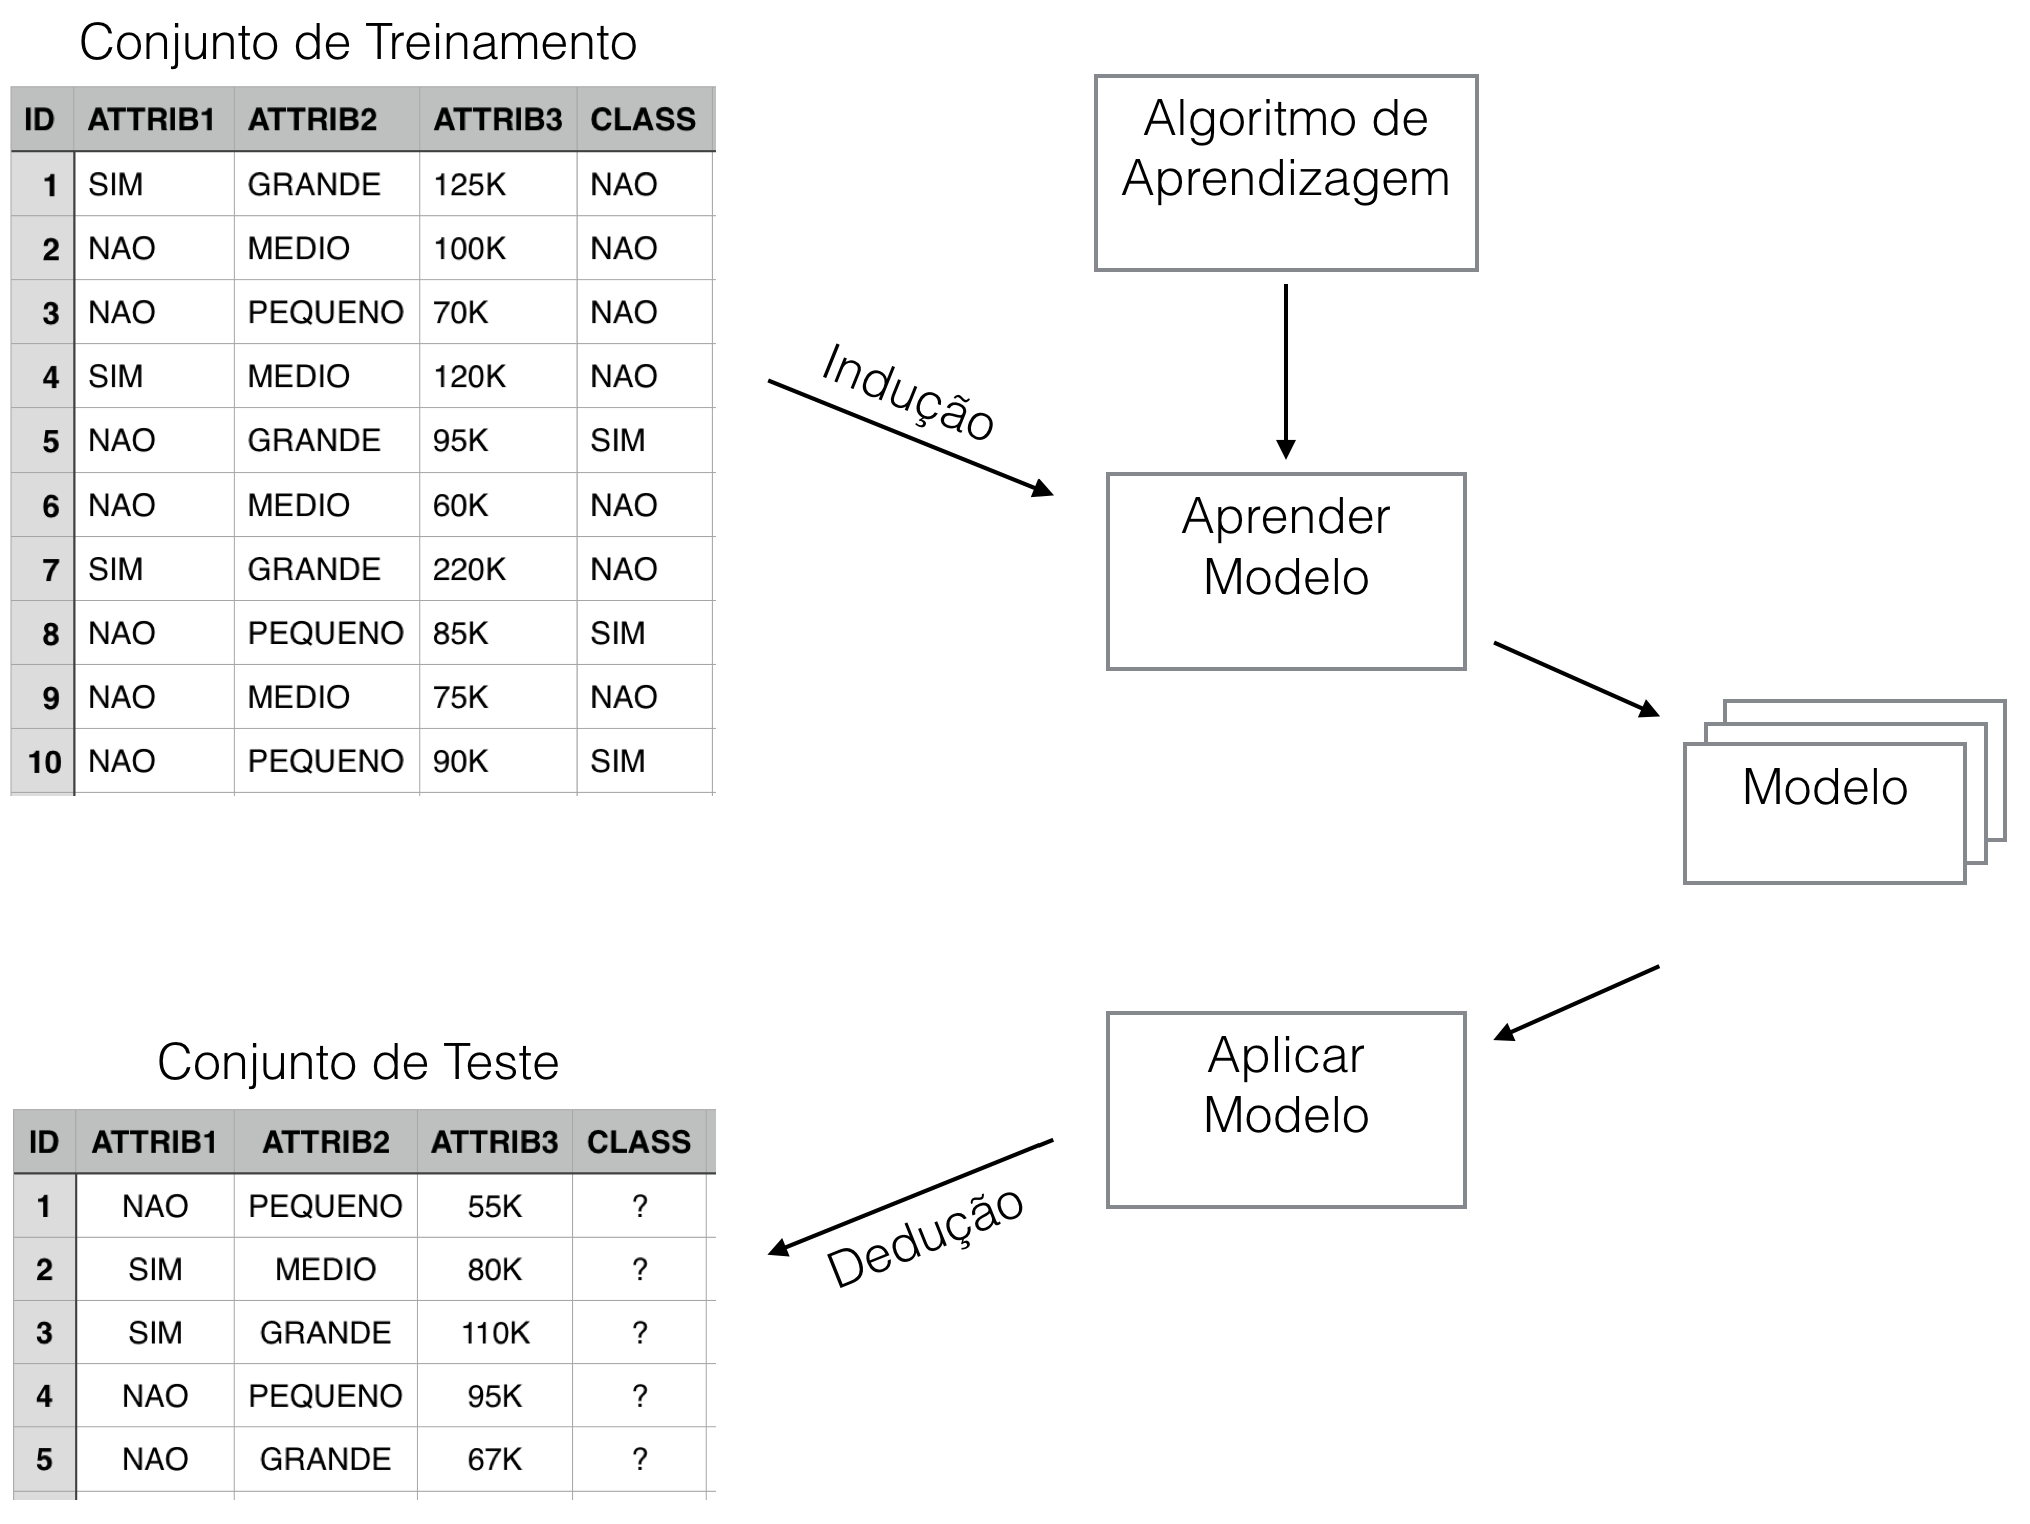
\includegraphics[scale=0.3]{img/abordagemModeloClassificacao.png}
			%			    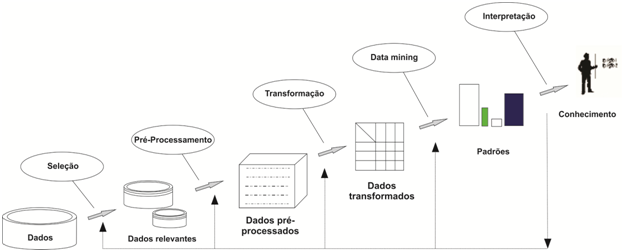
\includegraphics[scale=0.5]{img/dataMiningFayyad}
		\end{center}
		Fonte: \cite{tan:2009}.
	\end{figure}

	\subsection{Árvore de Decisão IMPORTANTE }
	
		Árvores de Decisão é, provavelmente, o algoritmo de AM mais estudado para apli- cações em Mineração de Dados (WITTEN; FRANK, 2000).
	
		Em uma árvore de decisão, cada nodo folha recebe um rótulo de classe. os nodos não terminais, que incluem o nodo raiz e outros nodos internos, contêm condições de testes de atributos para separar registros que possuem características diferentes.
		
		Classificar um registro de testes é direto, assim que uma árvore de decisão tenha sido construída. Começando do nodo raiz, aplicamos a condição de teste ao registro e seguimos a ramificação apropriada baseados no resultado do teste. Isto nos levará a um outro nodo interno, para o qual uma nova condição de teste é aplicada, ou a um nodo folha \cite{tan:2009}.
		
		Utilizamos os algoritmos: J48, RandomTree e REPTree.
		
	\subsection{Bayes}
	
	Em muitas aplicações, o relacionamento entre o conjunto de atributos e a variável classe é não determinístico. O rótulo da classe de um registro de teste não pode ser previsto com certeza embora seu conjunto de atributos seja idêntico a alguns dos exemplos de treinamento. Esta situação pode surgir por causa de dados com ruídos oud a presença de determinados fatores de confusão que afetam a classificação mas que não são incluídos na análise.
	
	O teorema de Bayes pode ser usado para resolver o problema de previsão.....
	
	Utilizamos o algoritmo NaiveBayes
	
	\subsection{Máquinas de Vetores de Suporte (SVM)}
	
	Uma técnica de classificação que tem recebido considerável atenção é esta técnica que possui seus fundamentos na teoria de aprendizagem estatística e tem mostrado resultados empíricos promissores em muitas aplicações práticas, desde o reconhecimento de dígitos escritos à mão até a categorização de textos. SVM também funciona bem com dados de alta dimensionalidade e evita o problema da dimensionalidade. Outro aspecto único desta abordagem é que ela representa o limite da decisão usando um subconjunto dos exemplos de treinamento, conhecido com vetores de suporte \cite{tan:2009}.
	
	Na Figura \ref{figsvmHiperPlanos}, existe um conjunto de classificadores lineares que separam duas classes, mas apenas um (em destaque) que maximiza a margem de separação (distância da instância mais próxima ao hiperplano de separação das classes). O hiperplano com margem máxima é chamado de hiperplano ótimo \cite{junior:2010}.
	\\
	\begin{figure}[!htb]
		\caption{\label{figsvmHiperPlanos} Conjunto de hiperplanos possíveis}
		\begin{center}
			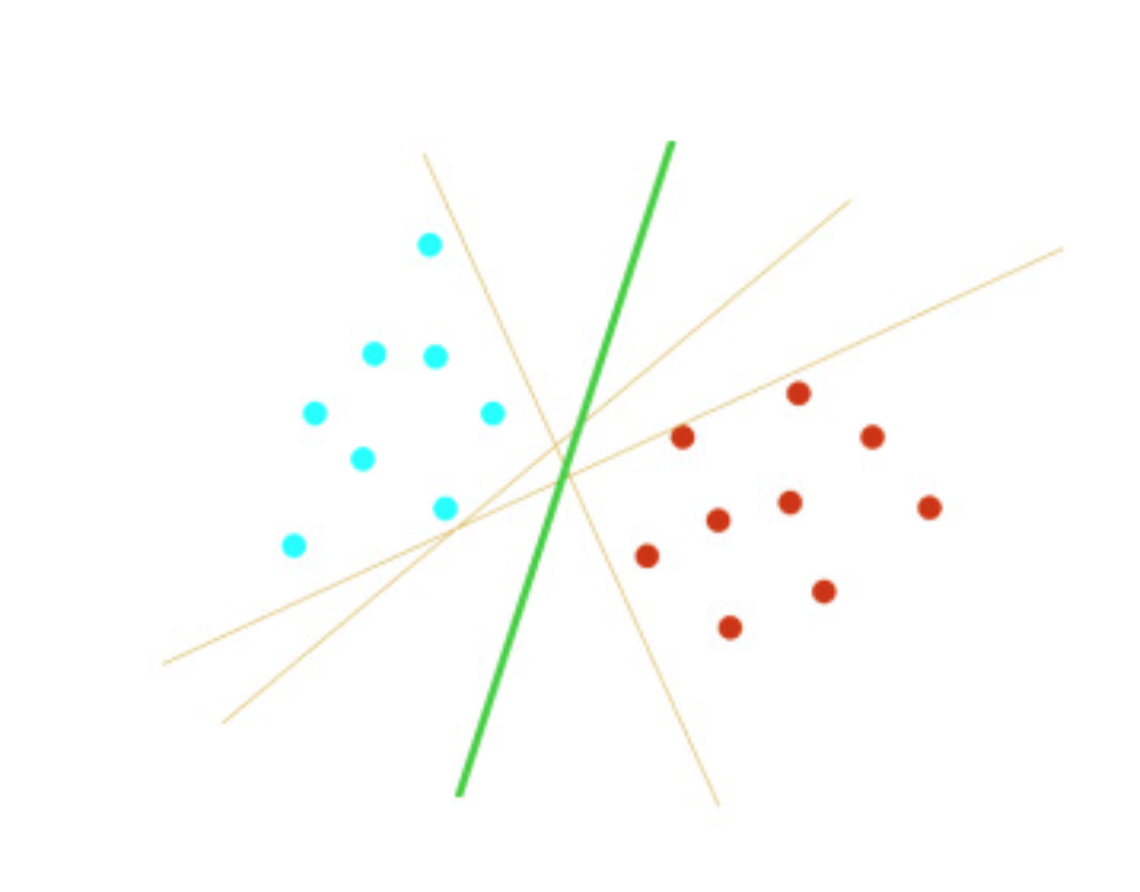
\includegraphics[scale=0.5]{img/svmHiperPlanos.png}
			%			    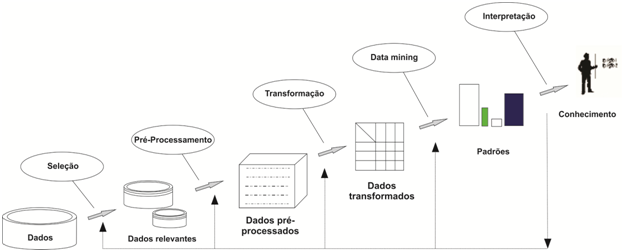
\includegraphics[scale=0.5]{img/dataMiningFayyad}
		\end{center}
		Fonte: \cite{junior:2010}.
	\end{figure}
	
	Utilizamos o algoritmo SMO.


	\section{WEKA}
% ---
% Capítulo 3
% ---
\chapter{Base de Dados}

	A base de dados utilizada foi a do Município de Fortaleza
	
	Neste capítulo, avaliamos os modelos gerados com os algoritmos que implementam a técnica de classificação através de um conjunto de experimentos.

	\begin{itemize}
		\item Metodologia de teste Cross-validation: Usa validação cruzada do tipo k-fold
	\end{itemize}

	
	\section{Dados Abertos}
	
	Utilizamos a base de dados disponibilizada pelo portal de dados abertos da prefeitura do Rio de Janeiro de casos notificados de dengue.

		\begin{table}[]
			\caption{Descrição dos atributos do conjunto de dados}
			\label{tabelaDescricaoAtributos}
			\centering
			\label{my-label}
			\begin{tabular}{@{}lllll@{}}
				\toprule
				Atributos            & Descrição                        &  &  &  \\ \midrule
				Data da investigação & Informar a data de investigação  &  &  &  \\
				Ocupação             & Informar ramo da ocupação        &  &  &  \\
				Classificação        & Informar a classificarão do caso &  &  &  \\ \bottomrule
			\end{tabular}
		\end{table}
		
		
	\section{SINAN}
	
		Nossos experimentos foram realizados a partir do conjunto de dados disponibilizado pela prefeitura do Rio de Janeiro do ano de 2015. Contendo inicialmente 26.568 instâncias e 97 atributos.
		Aplicamos os filtros: NumericToNominal -R 64, RemoveUseless -M 99.0. E observamos que a quantidade de atributos ficou igual a 66.
		Removemos os atributos: DT_NASC (ID 12), NU_DDD_TEL (ID 29), DDD_HOSP (ID 64), TEL_HOSP, (ID 65) NU_LOTE_I (ID 66), . Totalizando 61 atributos utilizados no experimento.
		Attribute a Class em CLASSI_FIN, para que que este atributo torne-se a classe rótulo
		Aplicamos o filtro RemoveRange -R $5001$-last, para realizarmos o experimento com $5.000$ instâncias e o atributo CLASSI_FIN com $22$\% das instâncias vazias.
		
		Aplicamos o filtro RemoveRange -R $10001$-last, para realizarmos o experimento com $10.000$ instâncias e o atributo CLASSI_FIN com $19$\% das instâncias vazias.
		
		Aplicamos o filtro RemoveRange -R $15001$-last, para realizarmos o experimento com $15.000$ instâncias e o atributo CLASSI_FIN com $19$\% das instâncias vazias.

		
% - - -
% Capítulo 4
% - - -
\chapter{Metodologia}

%	\section{Seção 1}
	
%		Teste de símbolo:
		
%		$\lambda$
		
%	\section{Seção 2}
	
%		Teste de abreviaturas:
		
% - - -
% Capítulo 5
% - - -
\chapter{Resultados}

	\section{Validação Cruzada IMPORTANTE}
	
	Portanto, a melhor abordagem para a Validação Cruzada é a utilização do método de k-partições. Neste método, o conjunto de dados é dividido em k partições (segundo Witten e Frank (2000)

	\section{Medida de Desempenho dos Algoritmos}
	
	As medidas de desepenho resultantes da classificação foram: 
	
	\begin{itemize}
		\item Correctly Classified Instances
		\item Incorrectly Classified Instances
		\item TP Rate
		\item FP Rate
		\item Precision
		\item Recall
		\item F-Measure
		\item ROC Area
	\end{itemize}
	
	\subsection{J48}
	
	\subsection{RandomTree}

	\subsection{REPTree}	

	\subsection{NaiveBayes}

	\subsection{SMO}

	
	\section{Resultados Comparativos Entre os Modelos}
	
		
\chapter{Conclusão}

	As considerações finais formam a parte final (fechamento) do texto, sendo dito de forma resumida (1) o que foi desenvolvido no presente trabalho e quais os resultados do mesmo, (2) o que se pôde concluir após o desenvolvimento bem como as principais contribuições do trabalho, e (3) perspectivas para o desenvolvimento de trabalhos futuros. O texto referente às considerações finais do autor deve salientar a extensão e os resultados da contribuição do trabalho e os argumentos utilizados estar baseados em dados comprovados e fundamentados nos resultados e na discussão do texto, contendo deduções lógicas correspondentes aos objetivos do trabalho, propostos inicialmente.

% ----------------------------------------------------------
% ELEMENTOS PÓS-TEXTUAIS
% ----------------------------------------------------------
\postextual
\Spacing{1.5}
% -----------------------------------------------------------------------------
% Referencias Bibliograficas
% -----------------------------------------------------------------------------

\bibliography{referencias}

% ----------------------------------------------------------
% Apêndices
% ----------------------------------------------------------

% ---
% Inicia os apêndices
% ---

%\begin{apendicesenv}

% ----------------------------------------------------------
%\chapter{Primeiro apêndice}
% ----------------------------------------------------------

%Os apêndices são textos ou documentos elaborados pelo autor, a fim de complementar sua argumentação, sem prejuízo da unidade nuclear do trabalho.

%\end{apendicesenv}

% Anexos
% ----------------------------------------------------------

% ---
% Inicia os anexos
% ---
\begin{anexosenv}

% ---
\chapter{Dicionário de dados - SINAN online}

Este anexo descreve todos os atrubutos presentes no SINAN
% ---

%inserindo todas as páginas
%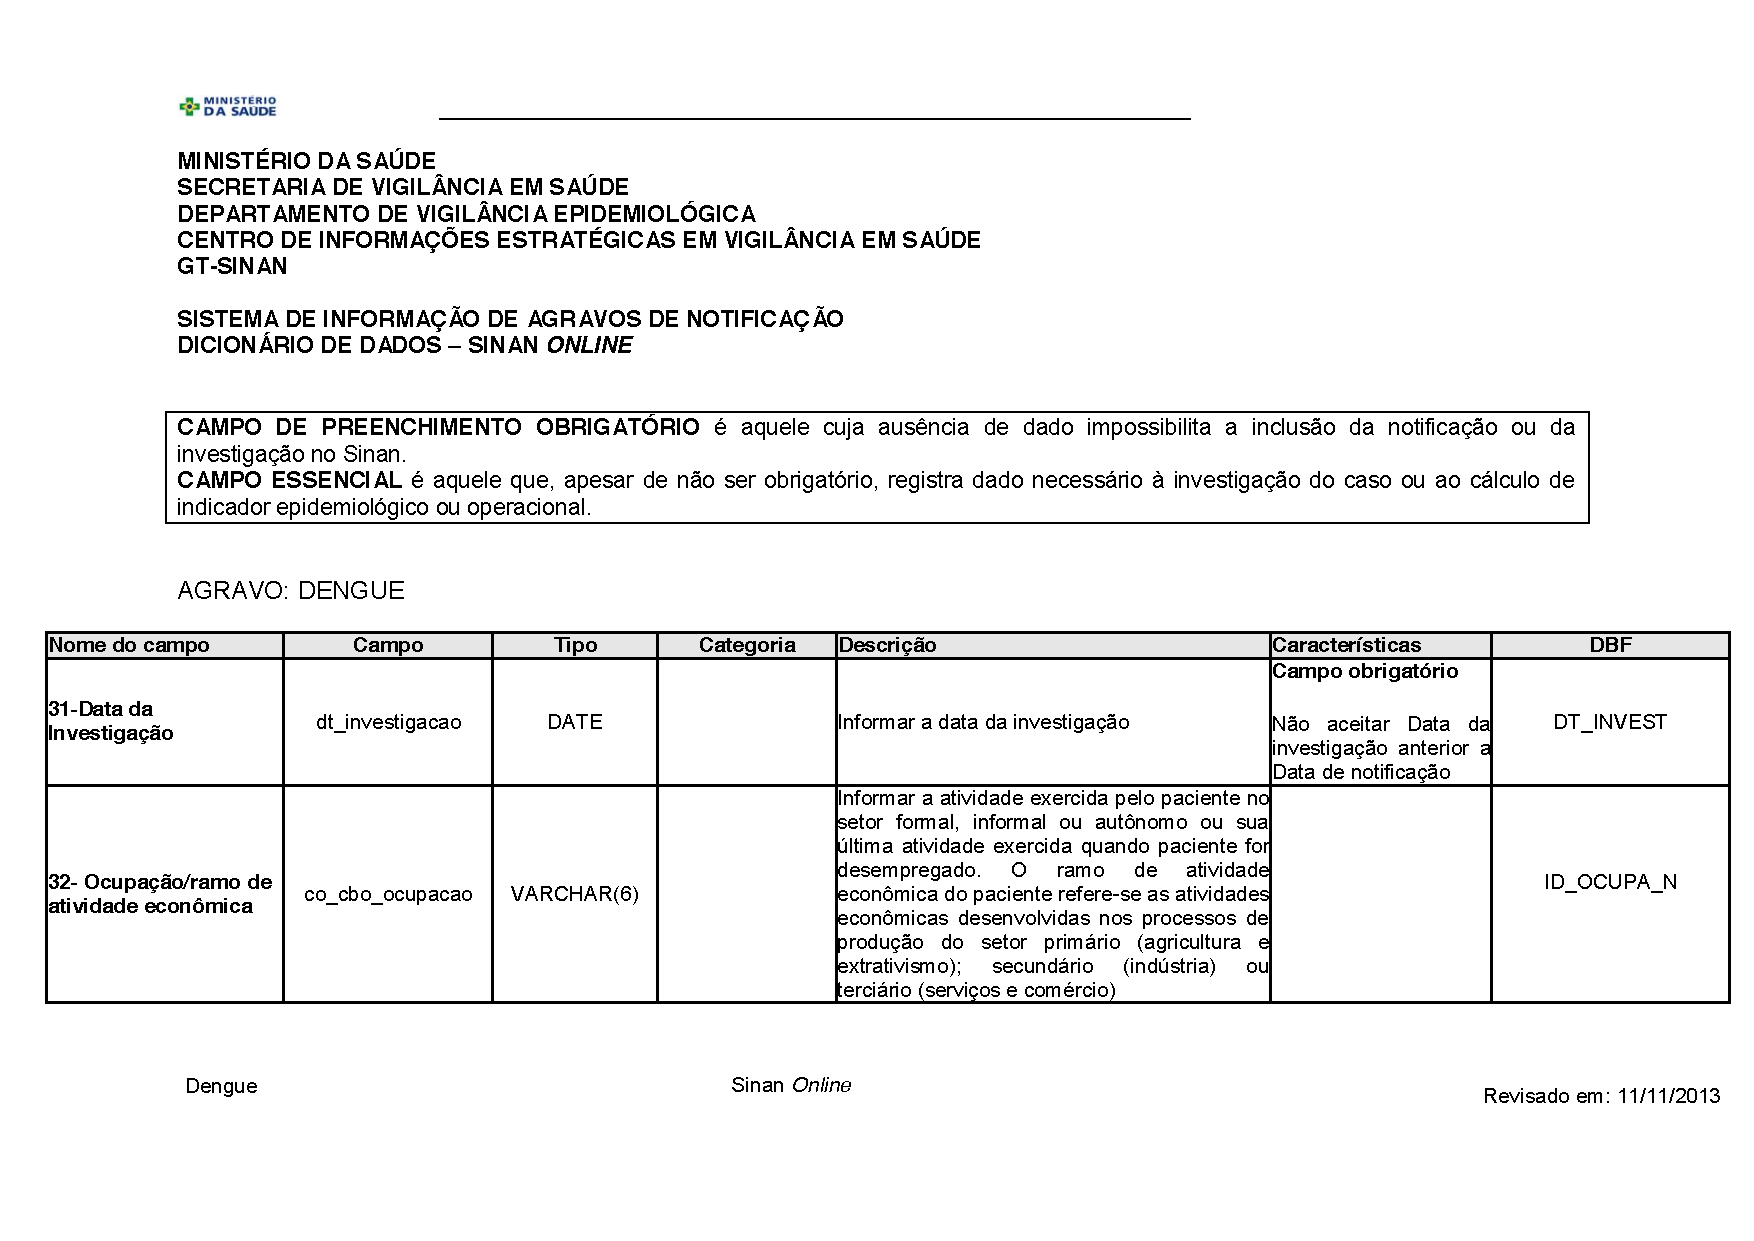
\includepdf[pages=-,landscape]{files/dicionarioDados.pdf}

\end{anexosenv}

\end{document}